\documentclass[tikz,border=4pt]{standalone}
\usepackage{amsmath}
\usetikzlibrary{arrows.meta,calc,decorations.pathmorphing,positioning}

\definecolor{sulfur}{HTML}{E3A500}
\definecolor{dib}{HTML}{4056A1}
\definecolor{charge}{HTML}{D94841}
\definecolor{energy}{HTML}{2A7F62}
\definecolor{ink}{HTML}{25313C}
\definecolor{panelbg}{HTML}{F7F9FA}

\tikzset{
  panel/.style={draw=ink!25, rounded corners=2pt, fill=panelbg, line width=0.6pt},
  atom/.style={circle, draw=ink, line width=0.55pt, minimum size=4.7mm,
    inner sep=0pt, font=\scriptsize\bfseries},
  apparatus/.style={draw=ink, rounded corners=1.5pt, fill=white,
    line width=0.65pt, align=center, font=\scriptsize},
  axis/.style={-Latex, draw=ink, line width=0.65pt},
  signal/.style={draw=energy, line width=1.1pt},
  charge/.style={circle, draw=charge, fill=charge!12, text=charge,
    minimum size=3.7mm, inner sep=0pt, font=\scriptsize\bfseries},
  flow/.style={-Latex, draw=ink!75, line width=0.7pt}
}

\newcommand{\paneltitle}[2]{%
  \node[anchor=north west, font=\bfseries\large, text=ink] at (0.18,4.28) {#1};
  \node[anchor=north west, font=\bfseries\small, text=ink] at (0.72,4.22) {#2};
}

\begin{document}
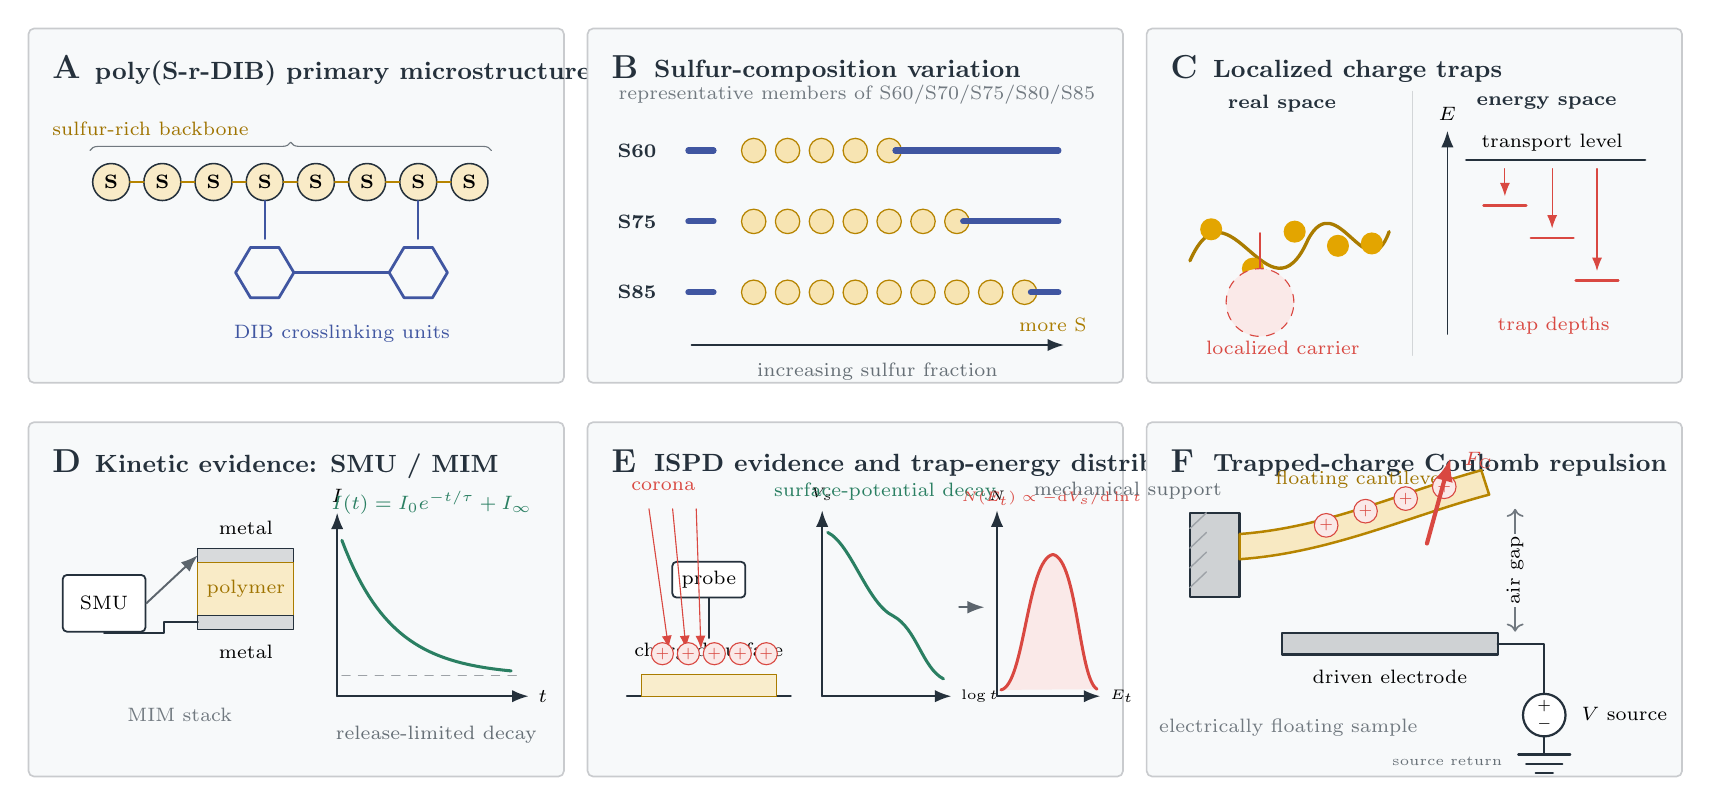
\begin{tikzpicture}[font=\sffamily, line cap=round, line join=round]

% Panel A: primary microstructure
\begin{scope}[shift={(0,5.0)}]
  \draw[panel] (0,0) rectangle (6.8,4.5);
  \paneltitle{A}{poly(S-r-DIB) primary microstructure}

  \foreach \x in {1.05,1.70,2.35,3.00,3.65,4.30,4.95,5.60}{
    \node[atom, fill=sulfur!22] at (\x,2.55) {S};
  }
  \foreach \x in {1.05,1.70,2.35,3.00,3.65,4.30,4.95}{
    \draw[thick, sulfur!80!black] (\x+0.24,2.55) -- (\x+0.41,2.55);
  }
  \draw[thick, dib] (3.00,2.31) -- (3.00,1.83);
  \draw[thick, dib] (4.95,2.31) -- (4.95,1.83);
  \draw[dib, line width=1pt] (2.63,1.40) -- (2.82,1.72) -- (3.18,1.72)
    -- (3.37,1.40) -- (3.18,1.08) -- (2.82,1.08) -- cycle;
  \draw[dib, line width=1pt] (4.58,1.40) -- (4.77,1.72) -- (5.13,1.72)
    -- (5.32,1.40) -- (5.13,1.08) -- (4.77,1.08) -- cycle;
  \draw[thick, dib] (3.37,1.40) -- (4.58,1.40);
  \node[font=\scriptsize, text=sulfur!70!black] at (1.55,3.23) {sulfur-rich backbone};
  \node[font=\scriptsize, text=dib] at (3.98,0.63) {DIB crosslinking units};
  \draw[decorate, decoration={brace, amplitude=3pt}, ink!65]
    (0.78,2.95) -- (5.88,2.95);
\end{scope}

% Panel B: composition series
\begin{scope}[shift={(7.1,5.0)}]
  \draw[panel] (0,0) rectangle (6.8,4.5);
  \paneltitle{B}{Sulfur-composition variation}
  \node[font=\scriptsize, text=ink!65] at (3.42,3.66)
    {representative members of S60/S70/S75/S80/S85};

  \foreach \y/\label/\n in {2.95/S60/5,2.05/S75/7,1.15/S85/9}{
    \node[anchor=east, font=\bfseries\scriptsize, text=ink] at (1.00,\y) {\label};
    \draw[dib, line width=2.2pt] (1.28,\y) -- (1.60,\y);
    \foreach \i in {1,...,\n}{
      \pgfmathsetmacro{\xx}{1.68+0.43*\i}
      \filldraw[fill=sulfur!30, draw=sulfur!80!black, line width=0.45pt]
        (\xx,\y) circle (1.55mm);
    }
    \pgfmathsetmacro{\xe}{1.76+0.43*\n}
    \draw[dib, line width=2.2pt] (\xe,\y) -- (5.98,\y);
  }
  \draw[axis] (1.32,0.48) -- (6.05,0.48);
  \node[anchor=north, font=\scriptsize, text=ink!70] at (3.68,0.38)
    {increasing sulfur fraction};
  \node[font=\scriptsize, text=sulfur!75!black] at (5.91,0.73) {more S};
\end{scope}

% Panel C: traps in real and energy space
\begin{scope}[shift={(14.2,5.0)}]
  \draw[panel] (0,0) rectangle (6.8,4.5);
  \paneltitle{C}{Localized charge traps}
  \draw[ink!20] (3.38,0.35) -- (3.38,3.70);
  \node[font=\bfseries\scriptsize, text=ink] at (1.72,3.55) {real space};
  \node[font=\bfseries\scriptsize, text=ink] at (5.08,3.55) {energy space};

  \draw[sulfur!75!black, line width=1.2pt]
    (0.55,1.55) .. controls (1.05,2.68) and (1.55,0.68) .. (2.05,1.82)
    .. controls (2.42,2.52) and (2.80,1.15) .. (3.08,1.92);
  \foreach \p in {(0.82,1.95),(1.35,1.45),(1.88,1.92),(2.43,1.74),(2.86,1.77)}
    \fill[sulfur] \p circle (1.4mm);
  \node[charge] (q1) at (1.44,1.02) {$-$};
  \draw[charge, -Latex, line width=0.8pt] (1.44,1.90) -- (q1.north);
  \draw[charge, dashed] (1.44,1.02) circle (4.3mm);
  \node[font=\scriptsize, text=charge] at (1.73,0.45) {localized carrier};

  \draw[axis] (3.82,0.62) -- (3.82,3.20) node[above, font=\scriptsize] {$E$};
  \draw[ink, line width=1pt] (4.06,2.83) -- (6.33,2.83);
  \node[anchor=west, font=\scriptsize] at (4.13,3.05) {transport level};
  \foreach \x/\yy in {4.55/2.25,5.15/1.84,5.72/1.30}{
    \draw[charge, line width=1pt] (\x-0.27,\yy) -- (\x+0.27,\yy);
    \draw[charge, -Latex] (\x,2.72) -- (\x,\yy+0.12);
  }
  \node[font=\scriptsize, text=charge] at (5.17,0.72) {trap depths};
\end{scope}

% Panel D: current-decay kinetics
\begin{scope}[shift={(0,0)}]
  \draw[panel] (0,0) rectangle (6.8,4.5);
  \paneltitle{D}{Kinetic evidence: SMU / MIM}

  \node[apparatus, minimum width=1.05cm, minimum height=0.72cm] (smu) at (0.96,2.20) {SMU};
  \draw[fill=ink!18, draw=ink] (2.15,2.72) rectangle (3.36,2.90);
  \draw[fill=sulfur!22, draw=sulfur!75!black] (2.15,2.05) rectangle (3.36,2.72);
  \draw[fill=ink!18, draw=ink] (2.15,1.87) rectangle (3.36,2.05);
  \draw[flow] (smu.east) -- (2.15,2.81);
  \draw[ink, line width=0.7pt] (2.15,1.96) -- (1.72,1.96) |- (smu.south);
  \node[font=\scriptsize] at (2.76,3.16) {metal};
  \node[font=\scriptsize, text=sulfur!70!black] at (2.76,2.38) {polymer};
  \node[font=\scriptsize] at (2.76,1.58) {metal};
  \node[font=\scriptsize, text=ink!65] at (1.92,0.78) {MIM stack};

  \draw[axis] (3.92,1.02) -- (6.35,1.02) node[right, font=\scriptsize] {$t$};
  \draw[axis] (3.92,1.02) -- (3.92,3.35) node[above, font=\scriptsize] {$I$};
  \draw[signal] plot[domain=0:2.15, samples=45]
    (3.98+\x,{1.28+1.72*exp(-1.55*\x)});
  \draw[ink!45, dashed] (3.98,1.28) -- (6.22,1.28);
  \node[font=\scriptsize, align=center, text=energy] at (5.12,3.48)
    {$I(t)=I_0e^{-t/\tau}+I_\infty$};
  \node[font=\scriptsize, text=ink!70] at (5.18,0.53) {release-limited decay};
\end{scope}

% Panel E: ISPD and inferred trap distribution
\begin{scope}[shift={(7.1,0)}]
  \draw[panel] (0,0) rectangle (6.8,4.5);
  \paneltitle{E}{ISPD evidence and trap-energy distribution}

  \draw[ink, line width=0.8pt] (0.50,1.02) -- (2.58,1.02);
  \draw[fill=sulfur!20, draw=sulfur!75!black] (0.68,1.02) rectangle (2.40,1.30);
  \node[font=\scriptsize, anchor=south] at (1.54,1.35) {charged surface};
  \node[apparatus, minimum width=0.72cm, minimum height=0.44cm] (probe) at (1.54,2.50) {probe};
  \draw[ink, line width=0.8pt] (probe.south) -- (1.54,1.76);
  \draw[charge, -Latex] (0.78,3.40) -- (1.03,1.62);
  \draw[charge, -Latex] (1.08,3.40) -- (1.25,1.62);
  \draw[charge, -Latex] (1.38,3.40) -- (1.44,1.62);
  \node[font=\scriptsize, text=charge] at (0.96,3.68) {corona};
  \foreach \x in {0.95,1.28,1.61,1.94,2.27}
    \node[charge, minimum size=2.8mm, font=\tiny] at (\x,1.56) {$+$};

  \draw[axis] (2.98,1.02) -- (4.62,1.02) node[right, font=\tiny] {$\log t$};
  \draw[axis] (2.98,1.02) -- (2.98,3.38) node[above, font=\tiny] {$V_s$};
  \draw[signal] (3.05,3.10) .. controls (3.35,2.95) and (3.55,2.20) ..
    (3.88,2.04) .. controls (4.18,1.88) and (4.25,1.38) .. (4.52,1.24);
  \node[font=\scriptsize, text=energy] at (3.78,3.62) {surface-potential decay};

  \draw[flow] (4.72,2.15) -- (5.04,2.15);
  \draw[axis] (5.20,1.02) -- (6.51,1.02) node[right, font=\tiny] {$E_t$};
  \draw[axis] (5.20,1.02) -- (5.20,3.38) node[above, font=\tiny] {$N$};
  \draw[charge, line width=1.1pt] (5.25,1.10) .. controls (5.55,1.16) and
    (5.58,2.76) .. (5.91,2.82) .. controls (6.22,2.76) and (6.24,1.24) .. (6.47,1.11);
  \node[font=\tiny, align=center, text=charge] at (5.89,3.53)
    {$N(E_t)\propto-\mathrm{d}V_s/\mathrm{d}\ln t$};
\end{scope}

% Panel F: floating cantilever repelled from driven electrode
\begin{scope}[shift={(14.2,0)}]
  \draw[panel] (0,0) rectangle (6.8,4.5);
  \paneltitle{F}{Trapped-charge Coulomb repulsion}

  % Mechanical restraint only: no electrical connection at the support.
  \draw[fill=ink!22, draw=ink, line width=0.8pt] (0.55,2.28) rectangle (1.18,3.35);
  \foreach \y in {2.40,2.65,2.90,3.15}
    \draw[ink!45, line width=0.5pt] (0.55,\y) -- (0.76,\y+0.20);
  \draw[fill=sulfur!24, draw=sulfur!80!black, line width=0.9pt]
    (1.18,2.76) .. controls (2.34,2.84) and (3.36,3.32) .. (4.35,3.58)
    -- (4.25,3.89) .. controls (3.20,3.60) and (2.28,3.16) .. (1.18,3.08) -- cycle;
  \node[font=\scriptsize, text=ink!70, anchor=east] at (1.08,3.63) {mechanical support};
  \node[font=\scriptsize, text=sulfur!70!black] at (2.74,3.77) {floating cantilever};
  \foreach \p in {(2.28,3.19),(2.78,3.37),(3.29,3.53),(3.78,3.68)}
    \node[charge, minimum size=3mm, font=\tiny] at \p {$+$};

  \draw[fill=ink!22, draw=ink, line width=0.9pt] (1.72,1.55) rectangle (4.46,1.82);
  \node[font=\scriptsize, anchor=north] at (3.09,1.48) {driven electrode};
  \draw[<->, ink!65, line width=0.6pt] (4.68,1.84) -- (4.68,3.40);
  \node[font=\scriptsize, rotate=90, fill=panelbg, inner sep=1pt] at (4.68,2.62) {air gap};

  \draw[-{Latex[length=3mm]}, charge, line width=1.5pt]
    (3.56,2.96) -- (3.86,4.05);
  \node[font=\scriptsize\bfseries, text=charge, anchor=west] at (3.91,4.02)
    {$F_{\mathrm C}$};

  \draw[ink, line width=0.8pt] (4.46,1.68) -| (5.05,1.05);
  \draw[ink, fill=white, line width=0.8pt] (5.05,0.78) circle (0.27);
  \node[font=\tiny] at (5.05,0.90) {$+$};
  \node[font=\tiny] at (5.05,0.67) {$-$};
  \node[font=\scriptsize, anchor=west] at (5.40,0.79) {$V$ source};
  \draw[ink, line width=0.8pt] (5.05,0.51) -- (5.05,0.28);
  \draw[ink, line width=0.8pt] (4.72,0.28) -- (5.38,0.28);
  \draw[ink, line width=0.8pt] (4.82,0.16) -- (5.28,0.16);
  \draw[ink, line width=0.8pt] (4.94,0.04) -- (5.16,0.04);
  \node[font=\tiny, text=ink!70, anchor=east] at (4.64,0.20) {source return};
  \node[font=\scriptsize, text=ink!65] at (1.80,0.62) {electrically floating sample};
\end{scope}

\end{tikzpicture}
\end{document}
